% Complementary Solutions Diagram - Professional Layout
% Complete redesign with proper spacing and modern layout

\begin{figure}[ht]
\centering
\begin{tikzpicture}[
    % Consistent styling with reduced overall scale and better spacing
    scale=0.77, % Further reduced for more space
    header/.style={font=\bfseries\sffamily\large, align=center, text width=9cm},
    mainbox/.style={rectangle, rounded corners=10pt, minimum width=5cm, 
                   minimum height=1.5cm, font=\bfseries\sffamily\large, 
                   text centered, text=white, inner sep=12pt},
    methodbox/.style={rectangle, rounded corners=8pt, minimum width=4.8cm,
                     minimum height=1.3cm, font=\sffamily, 
                     text centered, inner sep=10pt},
    featurebox/.style={rectangle, rounded corners=5pt, minimum width=4.8cm,
                      minimum height=2.6cm, font=\sffamily, 
                      align=left, inner sep=12pt},
    visualbox/.style={rectangle, rounded corners=5pt, minimum width=4.8cm,
                     minimum height=3.2cm, font=\sffamily, 
                     align=center, inner sep=12pt},
    commonbox/.style={rectangle, rounded corners=8pt, minimum width=10.5cm,
                     minimum height=1.4cm, font=\bfseries\sffamily,
                     text centered, inner sep=10pt},
    propbox/.style={rectangle, rounded corners=5pt, minimum width=10cm,
                   minimum height=3.6cm, font=\sffamily,
                   align=left, inner sep=15pt}
]

% Larger overall background with padding
\fill[white, rounded corners=15pt, draw=gray!10, line width=1pt] 
    (-7,-7.5) rectangle (7,6.5);

% Document title - more space at top and text width constraint
\node[header] at (0,5.8) {Complementary Solutions to\\Hermite's Problem};

% Main algorithm boxes - increased vertical separation
\node[mainbox, fill=blue!70] (hapd) at (-5,4.0) {HAPD Algorithm};
\node[mainbox, fill=red!70] (sin) at (5,4.0) {Modified sin$^2$ Algorithm};

% Complementary methods arrow - adjusted for spacing
\draw[<->, very thick, purple!70] (hapd.east) -- (sin.west) 
    node[midway, above, font=\sffamily, fill=white, inner sep=5pt] {Complementary methods};

% Approach methods - more vertical spacing between elements
\node[methodbox, fill=blue!10, draw=blue!30] (hapd_app) at (-5,2.2) {Non-subtractive approach};
\node[methodbox, fill=red!10, draw=red!30] (sin_app) at (5,2.2) {Subtractive approach};

% Features boxes - increased height and spacing between bullet points
\node[featurebox, fill=blue!5, draw=blue!20] (hapd_feat) at (-5,-0.2) {
    \begin{itemize}[leftmargin=12pt, itemsep=8pt]
        \item Projective space $\mathbb{RP}^2$
        \item Matrix-based approach
    \end{itemize}
};

\node[featurebox, fill=red!5, draw=red!20] (sin_feat) at (5,-0.2) {
    \begin{itemize}[leftmargin=12pt, itemsep=8pt]
        \item Complex plane analysis
        \item Transcendental terms
    \end{itemize}
};

% Visual representations - increased height and better internal spacing
\node[visualbox, fill=blue!5, draw=blue!20] (hapd_vis) at (-5,-3.2) {
    \textbf{Projective dynamics}\\[0.7cm]
    \begin{tikzpicture}[scale=0.6]
        \draw[->, thick, blue] (-1.5,0) -- (1.5,0) node[right] {$x$};
        \draw[->, thick, blue] (0,-0.8) -- (0,1) node[above] {$y$};
        \draw[blue, thick] (0,0) circle (0.7cm);
        \draw[->, blue, thick] (0.7,0) arc(0:60:0.7);
    \end{tikzpicture}
};

\node[visualbox, fill=red!5, draw=red!20] (sin_vis) at (5,-3.2) {
    \textbf{sin$^2$-weighting}\\[0.7cm]
    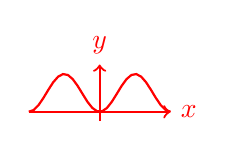
\begin{tikzpicture}[scale=0.6]
        \draw[->, thick, red] (-1.5,0) -- (1.5,0) node[right] {$x$};
        \draw[->, thick, red] (0,-0.2) -- (0,1) node[above] {$y$};
        \draw[red, thick] plot[domain=-1.5:1.5, samples=30] 
            (\x, {0.8*sin(120*\x)*sin(120*\x)});
    \end{tikzpicture}
};

% Common properties - more vertical space from visuals above
\node[commonbox, fill=gray!15, draw=gray!40] (common) at (0,-5.6) {Common Properties};

% Properties box - taller with more internal spacing
\node[propbox, fill=white, draw=gray!20] (properties) at (0,-7.0) {
    \begin{itemize}[leftmargin=18pt, itemsep=10pt]
        \item Periodic precisely for cubic irrationals
        \item Handle complex conjugate roots
        \item Theoretical guarantees
        \item Numerical validation
    \end{itemize}
};

% Connect to common properties - adjusted for new positions and wider spacing
\draw[->, thick, blue!50] (-5,-4.8) -- (-3,-5.6);
\draw[->, thick, red!50] (5,-4.8) -- (3,-5.6);

\end{tikzpicture}
\caption{Comparison of complementary approaches to Hermite's problem. The HAPD algorithm uses a non-subtractive approach in projective space (left), while the Modified sin$^2$ algorithm employs a subtractive approach with transcendental functions (right). Both methods effectively detect periodicity in cubic irrationals.}
\label{fig:complementary_approaches}
\end{figure} 